\documentclass[output=paper]{../langscibook}
\ChapterDOI{10.5281/zenodo.4449770}
\author{Ana Carvalho\affiliation{University of Arizona}}
\title{A close look at how context of acquisition of previous languages influences third language pedagogy: Does one model fit all?}

\abstract{}



\IfFileExists{../localcommands.tex}{
  \addbibresource{../localbibliography.bib}
  \usepackage{langsci-optional}
\usepackage{langsci-gb4e}
\usepackage{langsci-lgr}

\usepackage{listings}
\lstset{basicstyle=\ttfamily,tabsize=2,breaklines=true}

%added by author
% \usepackage{tipa}
\usepackage{multirow}
\graphicspath{{figures/}}
\usepackage{langsci-branding}

  
\newcommand{\sent}{\enumsentence}
\newcommand{\sents}{\eenumsentence}
\let\citeasnoun\citet

\renewcommand{\lsCoverTitleFont}[1]{\sffamily\addfontfeatures{Scale=MatchUppercase}\fontsize{44pt}{16mm}\selectfont #1}
   
  %% hyphenation points for line breaks
%% Normally, automatic hyphenation in LaTeX is very good
%% If a word is mis-hyphenated, add it to this file
%%
%% add information to TeX file before \begin{document} with:
%% %% hyphenation points for line breaks
%% Normally, automatic hyphenation in LaTeX is very good
%% If a word is mis-hyphenated, add it to this file
%%
%% add information to TeX file before \begin{document} with:
%% %% hyphenation points for line breaks
%% Normally, automatic hyphenation in LaTeX is very good
%% If a word is mis-hyphenated, add it to this file
%%
%% add information to TeX file before \begin{document} with:
%% \include{localhyphenation}
\hyphenation{
affri-ca-te
affri-ca-tes
an-no-tated
com-ple-ments
com-po-si-tio-na-li-ty
non-com-po-si-tio-na-li-ty
Gon-zá-lez
out-side
Ri-chárd
se-man-tics
STREU-SLE
Tie-de-mann
}
\hyphenation{
affri-ca-te
affri-ca-tes
an-no-tated
com-ple-ments
com-po-si-tio-na-li-ty
non-com-po-si-tio-na-li-ty
Gon-zá-lez
out-side
Ri-chárd
se-man-tics
STREU-SLE
Tie-de-mann
}
\hyphenation{
affri-ca-te
affri-ca-tes
an-no-tated
com-ple-ments
com-po-si-tio-na-li-ty
non-com-po-si-tio-na-li-ty
Gon-zá-lez
out-side
Ri-chárd
se-man-tics
STREU-SLE
Tie-de-mann
} 
  \togglepaper[1]%%chapternumber
}{}

\maketitle
\shorttitlerunninghead{A close look at contexts of acquisition of previous languages}
\begin{document}
\vspace{-2\baselineskip}
\begin{quote}\small
 {A significant proportion of college students in the United States have Spanish in their linguistic repertoire. Several language programs capitalize on these students’ bilingual skills to offer them the opportunity to develop proficiency in additional languages, especially cognate systems that can be acquired faster, such as French, Italian, and Portuguese. In this article, I first offer a synopsis of the research that has been developed on the acquisition of cognate languages in general, and the acquisition of Portuguese by Spanish speakers in particular. I then focus on the main premises that are considered in the curriculum designed to teach Portuguese for Spanish speakers in educational settings in the United States, pinpointing a tendency to treat Spanish speakers as a homogeneous group. Finally, I focus on incipient research that points to differences in patterns of L3 acquisition by learners who speak Spanish as their first, second, or heritage language, and problematize the assumption that they make up a homogeneous group with similar pedagogical needs.

  While possible differences among L3 learners due to different contexts of acquisition of previous languages have been pointed out by previous research, only a few studies have investigated these dissimilarities. This article aims to contribute to this growing area of research by exploring important differences among English-Spanish bilingual learners of L3 Portuguese who acquired Spanish as their L2 or heritage language both in terms of their performance in class and in terms of their perception of the learning process through an examination of previous studies and incipient survey data. It concludes that while L2 Spanish speakers benefit more from explicit teaching due to previous experience as language learners that lead to a higher level of metalinguistic awareness, heritage Spanish speakers are less fluent in metalinguistic terminology and an explicit understanding of grammar, and as such benefit from more implicit, naturalistic activities that rely on their intuition. Lastly, a number of important implications for curricular adjustments that cater for both types of Spanish speakers in L3 Portuguese classes are offered.}
\end{quote}

 \section{Introduction}

Given that an important population of English-speaking college students in the United States also speak Spanish, several language programs are capitalizing on these students’ bilingual skills by offering them opportunities to develop proficiency in additional languages, especially cognate systems that can be acquired easily and quickly. In this chapter, after establishing the substantial presence of Spanish speakers in higher education in the United States, I offer a synopsis of current research on the acquisition of Portuguese as a third language (L3) by Spanish-English bilinguals, and of the main premises that are considered in the curriculum designed to teach these students. As I show, there is a generalized but inaccurate tendency to treat Spanish speakers as a homogeneous group. Incipient research points to differences in patterns of L3 acquisition depending on whether learners were born in Spanish-speaking countries (L1 Spanish speakers), learned Spanish as adults in school settings (L2 Spanish speakers), or were early bilinguals who were born and raised in the United States but learned Spanish in their homes and communities (heritage Spanish speakers). By pinpointing important differences in the way these groups acquire additional languages, I problematize the assumption that “Spanish speakers” enrolled in L3 Portuguese classes are a uniform group with similar pedagogical needs. Finally, I stress the need to create a more inclusive L3 pedagogy and suggest curricular adjustments that would cater to all types of Spanish speakers enrolled in Portuguese courses, including heritage Spanish speakers.

Although possible differences among L3 learners due to different contexts of acquisition of previous languages have been identified by previous research (\citealt{Carvalho2002}; \citealt{Cenoz2011}; \citealt{Johnson2004}), only a few studies have investigated these dissimilarities (\citealt{CarvalhoChild2018}; \citealt{CarvalhoSilva2006}; \citealt{Child2014}, among others). Thus, in this chapter I contribute to a growing area of research by exploring systematic differences among English-Spanish bilingual learners of L3 Portuguese who acquired Spanish as their L2 versus as a heritage language, in terms of both their performance in class and their perception of the learning process. I conclude that L2 Spanish speakers benefit from explicit teaching because they have previous experience as language learners, whereas heritage Spanish speakers are less fluent in metalinguistic terminology and explicit understanding of grammar, and consequently benefit from more implicit, naturalistic activities that rely on their intuitive knowledge.

 \section{Spanish speakers in US higher education}


The United States has the fifth largest Spanish-speaking population in the world, after Mexico, Colombia, Spain, and Argentina (\citealt{EscobarPotowski2015}). This population has been growing steadily and more than 40 million inhabitants now claim Spanish as their home language (\figref{fig:3:1}), far exceeding speakers of other languages (\figref{fig:3:2}).



\begin{figure}
\footnotesize
  \begin{tikzpicture}
    \begin{axis}[
      axis lines*=left,
      nodes near coords={\pgfmathprintnumber[fixed]\pgfplotspointmeta},
      every node near coord/.append style={font=\footnotesize},
      width=1\textwidth,
      height=.2\textheight,
      ymin=36000000,
      ymax=42000000,
      xmin=2010.5,
      xmax=2016.5,
      ticklabel style={/pgf/number format/fixed,/pgf/number format/precision=5}, 
      scaled ticks=false,
      xtick=data,
      xticklabel style= {/pgf/number format/1000 sep=},
]
\addplot [black,mark=*] coordinates {
                                (2011,37579787) 
                                (2012,38325155)
                                (2013,38417235)
                                (2014,39254342)
                                (2015,40045795)
                                (2016,40489813)
                              };
\end{axis}
\end{tikzpicture}
\caption{Spanish speakers in the United States. Original source: US Census Bureau 2011--2016\label{fig:3:1}}
\end{figure}

\begin{figure}
  \includegraphics[width=.9\textwidth]{figures/Chapter3-img002.png}
  \caption{Languages other than English spoken in the US. Original source: US Census Bureau 2008--2016}
  \label{fig:3:2}
\end{figure}

\clearpage
While Spanish use is widespread throughout the United States, it is clear that the highest concentration occurs in the US south-west. In Arizona, the site of this study, more than 23\% of the population speaks Spanish as their first language (\figref{fig:3:3}).

\begin{figure}
  \includegraphics[width=\textwidth]{figures/Chapter3-img003.png}
  \caption{Map showing percentages of Spanish speakers in the US.  Reprinted by permission of the Modern
Language Association of America (www.mla.org), MLA Language Map, \url{https://www.mla.org/Resources/Research/MLA-Language-Map.}}
  \label{fig:3:3}
\end{figure}


A fraction of these speakers attends the University of Arizona, which earned the designation of a Hispanic-serving institution (HSI) in 2018, when Hispanic enrollment in its undergraduate programs exceeded 25\% (\figref{fig:3:4}).

 

\begin{figure}
\footnotesize
  \begin{tikzpicture}
    \begin{axis}[
      axis lines*=left,
      nodes near coords={\pgfmathprintnumber[fixed]\pgfplotspointmeta\%},
      width=1\textwidth,
      height=.3\textheight,
      ymin=0,
      ymax=30,
      ticklabel style={/pgf/number format/fixed,/pgf/number format/precision=5},
      scaled ticks=false,
      ytick distance = 5,
      xtick=data,
      xticklabels = {2009, 2010, 2011, 2012, 2013, 2014, 2015, 2016, 2017},
      legend pos = south east,
      legend columns=-1
        ]

\addplot [black,mark=*] coordinates {(1,10.32)(2,10.37)(3,10.18)(4,9.96)(5,11.31)(6,12.49)(7,13.83)(8,14.41)(9,15.04)}; \addlegendentry{Graduate}
\addplot [black,dashed,mark=*] coordinates {(1,17.80)(2,19.17)(3,20.99)(4,22.30)(5,24.36)(6,25.19)(7,25.33)(8,25.85)(9,26.54)};\addlegendentry{Undergraduate}
\end{axis}
\end{tikzpicture}
  \caption{Hispanic student percentages at the University of Arizona (Fall terms). Original source: University of Arizona's Fact Book}
    \label{fig:3:4}
\end{figure}
%\end{stylecaption}

The University of Arizona’s HSI status opens new opportunities to boost\linebreak grants and research collaborations. In addition, and crucially, this new status holds administrators and faculty -- including language educators and applied linguists~-- responsible for addressing this population’s needs, an important objective of the present study.

In addition to the students who acquire Spanish as their first or their heritage language, thousands of college students study Spanish as a second language. Spanish is by far the most popular language studied in schools; according to the latest Modern Language Association (MLA) 2016 report, half the students enrolled in foreign language courses are studying Spanish (\figref{fig:3:5}). Thus, a significant proportion of postsecondary students have Spanish in their linguistic repertoire, whether as a first, second, or heritage language.


\begin{table}[b]
    \sisetup{group-digits=true, group-separator={,}, group-minimum-digits=4}
    \fittable{\begin{tabular}{l *{2}{S[table-format=6.0]}@{\,}>(r<) S[table-format=6.0]@{\,}>(r<)S[table-format=6.0]@{\,}>(r<)}
      \lsptoprule
      & {2006} & \multicolumn{2}{c}{2009} &   \multicolumn{2}{c}{2013}  	& \multicolumn{2}{c}{2016}\\\midrule
    Spanish & 822148 & 861015 &	 +4.7 & 	789888 &	 –8.3 & 	712240 &	 –9.8 \\
    French & 	206019 &	 215244 &	 +4.5 & 	197679 &	 –8.2 & 	175667 &	 –11.1\\ 
    American Sign Language &	 79744 &	 92068 &	 +15.5 & 	109567 &	 +19.0&  	107060 	& –2.3\\ 
    German  &	94146 & 	 95613 &	 +1.6 & 	86782& 	 –9.2 & 	80594 &	 –7.1\\ 
    Japanese & 	65410& 	 72357 &	 +10.6 & 	66771 &	 –7.7 & 	68810 &	 +3.1\\ 
    Italian  &	78176& 	 80322 &	 +2.7 & 	70982& 	 –11.6 & 	56743 &	 –20.1\\ 
    Chinese  &	51382 &	 59876 &	 +16.5 & 	61084 &	 +2.0 & 	53069 &	 –13.1 \\
    Arabic\footnote{Includes enrollments reported under “Arabic”, “Arabic Algerian”, “Arabic Classical”, “Arabic Egyptian”, “Arabic Gulf”, “Arabic Iraqi”, “Arabic Levantine”, “Arabic Modern Standard”, “Arabic Moroccan,” “Arabic, Qur’anic,” “Arabic, Sudanese,” and “Arabic, Syrian.”}  &	24010 &	 35228 &	 +46.7 & 	33526 &	 –4.8 & 	31554& 	 –5.9 \\
    Latin  &	32164 &	 32446 &	 +0.9  &	27209 &	 –16.1  &	24866 &	 –8.6\\ 
    Russian  &	24784 &	 26740 &	 +7.9 & 	21979 &	 –17.8  &	20353 &	 –7.4\\ 
    Korean & 	7146 &	 8449 &	 +18.2 & 	12256 &	 +45.1 & 	13936 &	 +13.7\\ 
    Greek, Ancient\footnote{Includes enrollments reported under “Greek, Ancient,” “Greek, Biblical,” “Greek, Koine,” “Greek, New Testament,” and “Greek, Old Testament.” Excludes enrollments reported under “Greek,” “Greek and Hebrew,” and “Greek and Latin.”}  &	22842 &	 21515 &	 –5.8 & 	16961 &	 –21.2  &	13264 &	 –21.8\\ 
    Portuguese  &	10310 &	 11273 &	 +9.3 & 	12407 &	 +10.1 &	 9827 &	 –20.8 \\
    Hebrew, Biblical\footnote{Includes enrollments reported under “Hebrew, Biblical,” “Hebrew, Classical,” and “Hebrew, Rabbinic.” Excludes enrollments reported under “Hebrew” and “Hebrew, Biblical and Modern.”}  &	14137 &	 13764 &	 –2.6 & 	12596 &	 –8.5 &	 9587 &	 –23.9\\ 
    Hebrew Modern  &	9620 &	 8307 &	 –13.6 &	 6698 &	 –19.4 &	 5521 &	 –17.6\\ 
    Other Languages  &	33800 &	 39349 &	 +16.4 & 	34746 &	 –11.7  &	34747 &	 +0.0\\ \midrule
    Total & 	1575838 &	 1673566 &	 +6.2 & 	1561131 	& –6.7  &	1417838 &	 –9.2\\\lspbottomrule
\end{tabular}}
  \caption{Language (other than English) enrollments and percentage change to the previous date as reported by the MLA. Original source: MLA Report 2016\label{fig:3:5}}%\todo[inline]{Please get in touch if you want the same coloring as the original table.}
\end{table}

These students’ bilingual skills can accelerate their proficiency in additional languages, especially cognate systems such as French, Italian, and Portuguese. Spanish-English bilingual students who study cognate languages have an exceptional opportunity to become trilingual, in accordance with the Modern Language Association’s recommendation that higher education should promote\linebreak “speakers who have deep translingual and transcultural competence” \citep[7]{MLA2007}.

 \section{Portuguese for Spanish speakers}


In fact, the substantial presence of Spanish speakers in the US education system has prompted several initiatives to encourage Spanish-English bilinguals to learn additional languages. For example, Donato and her associates (\citealt{DonatoOliva2015}; \citealt{DonatoPasquarelli-Gascon2015}) have successfully implemented French and Italian language courses for Spanish speakers in high schools and colleges across greater Los Angeles. At the postsecondary level, the growth of Portuguese courses for Spanish speakers has driven a rapid increase in enrollment in Portuguese programs nationwide \citep[14]{Milleret2012}. In a survey of postsecondary Portuguese programs in the United States, almost half (50 of 107 responding institutions offered a beginning-level Portuguese course specifically for Spanish speakers, \citealt{BatemanOliveira2014}). These courses capitalize on the fact that cognate languages can be acquired rapidly and efficiently. As \citet{Wiedemann2009} showed, Spanish speakers on average can learn Portuguese in half the time as English monolinguals because they have a high level of receptive skills from the beginning. Spanish speakers with no previous knowledge of Portuguese can understand more than 50\% of what is said in standard Portuguese \citep{Jensen1989}. Written words are even more transparent. \citet{Henriques2000} found that monolingual Spanish speakers could comprehend up to 94\% of the content of academic texts written in Portuguese, due to the very high degree of lexical similarity between the languages.

Thus, positive transfer translates into advanced receptive skills, which lessens students’ affective filter, decreases their anxiety level, increases their motivation to learn a cognate language, and serves as an effective recruiting strategy to attract bilingual students into adding another language to their repertoire relatively quickly. These advantages are, however, counterbalanced by a predisposition to non-felicitous transfer, since cross-linguistic transfer occurs at all levels of the grammar and is believed to induce early fossilization of an interlanguage because students are able to communicate basic meanings early in the learning process (\citealt{SimoesKelm1991}; \citealt{Takeuchi1984}; \citealt{CarvalhoEtAl2010}, among others). Even though non-facilitative and facilitative transfer processes are interconnected, and positive transfer is a crucial facilitating factor in the acquisition process, pedagogy has emphasized combating non-facilitative transfer (\citealt{Carvalho2002}; \citealt{CarvalhoChild2018}). In fact, the most common pedagogical techniques aim at developing metalinguistic awareness, an approach considered to support control of multilingual processing (\citealt{Jessner2006}: 106). Through both contrastive analysis and focus on form, students are expected to learn to discern subtle but important differences and similarities between cognate languages, and crucially, to capitalize on the similarities while avoiding transfer of the differences. Thus, most curricula available in the United States emphasize cross-metalinguistic awareness by comparing the languages based on the learners’ declarative knowledge of Spanish and their baseline knowledge of Portuguese. 

Three textbooks available in the United States are designed for Spanish speakers who are learning Portuguese \citep{Simoes1992,Simoes2010,BatemanEtAl2016}; there are also several online resources, including a podcast\footnote{\url{https://www.coerll.utexas.edu/brazilpod/tafalado/}}. All these resources emphasize differences and similarities between the languages so that the student can use this knowledge to learn by analogy and generalization. Focusing on formal differences, these materials target classroom practice and pedagogical strategies that emphasize metalinguistic explanations and contrastive discussions that elicit declarative knowledge. The facilitation of metalinguistic awareness is believed to help learners recognize degrees of crosslinguistic relationships, capitalize on similarities, and avoid differences (cross-linguistic interference). 

As Portuguese for Spanish speakers courses and instructional materials multiplied, curriculum developers and linguists began to engage in research to elucidate the particular processes involved in learning cognate languages, in order to inform teaching practices and curriculum design. Several symposia were organized, leading to the publication of selected proceedings \citep{SimoesEtAl2004,WiedemannScaramucci2008} that accompanied a call for research in a field that was heavily based on contrastive analysis \citep{Carvalho2002}. Over the past 15 years experimental research on English-Spanish bilinguals’ acquisition of L3 Portuguese has flourished (\citealt{Allegro2010}; \citealt{Bailey2013}; \citealt{FeidenEtAl2014}; \citealt{Silva2015}; \citealt{TrudeTokowicz2011}, among others). In all cases, research results corroborate that as Spanish-English bilinguals learn Portuguese, transfer from Spanish is inevitable. This body of research yields to two broad generalizations. First, linguistic overlap is the strongest predictor of transfer, as predicted by \citegen{Rothman2010} typological premise model. Second, it presupposes that bilinguals are a homogenous group of learners, regardless of the different contexts in which they acquired their previous languages, a generalization that \citet{Carvalho2002} and \citet{Cenoz2011} have questioned. As Cenoz (2011: 80) states, it “may be a mistake not to be aware of the important difference between both types (active bilinguals and foreign language users) or to ignore the implications of dealing with one situation rather than the other.” In fact, acquisitionist studies that follow the formal tradition have identified different transfer patterns which correlate with the order of acquisition of previous languages (\citealt{CabrelliAmaroWrembel2016}; \citealt{ChildEtAl2017}; \citealt{Silva2015}; \citealt{GiancasproEtAl2015}; \citealt{Rothman2010}, among others). Meanwhile, \citet{CarvalhoSilva2006}, \citet{CarvalhoChild2018}, and \citet{KoikeFlanzer2004} have analyzed how Spanish speakers’ backgrounds influence how they learn the L3. More specifically, these authors argue, with \citet{Cenoz2011}, that it is important to consider the distinctions between L2 Spanish speakers’ previous experience of learning a language in a school setting versus heritage Spanish speakers’ experiences of acquiring Spanish in naturalistic environments. These differences have direct implications for teaching methods, as I discuss below.

 \section{L3 Portuguese acquisition by speakers of Spanish as L1, L2, and Heritage Language (HL)}


A brief survey at the University of Arizona, a large public university in the US Southwest, revealed that almost half the students enrolled in Fall 2018 Portuguese classes were heritage Spanish speakers who reported being “exposed to Spanish as a child in their household” (\figref{fig:3:6}, adapted from \citealt{Sommer-FariasEtAl2020}). The second largest group was L2 Spanish speakers, or students who learned Spanish in a school setting (28.3\%), followed by L1 Spanish speakers, or students who were born in a Spanish-speaking country, in this case, typically Mexico. Less than 5\% of students did not speak Spanish. Similar tendencies are evident in other universities in the US Southwest that offer Portuguese for Spanish speakers (see, for example, \citealt{Milleret2012}).

  
%%please move the includegraphics inside the {figure} environment
%%\includegraphics[width=\textwidth]{figures/Chapter3-img006.png}
 

\begin{figure}
  \begin{tikzpicture}
    \begin{axis}[ybar,
        width=1\textwidth,
        height=.3\textheight,
        ymin=0,
        ymax=60,
        ytick={0,10,20,30,40,50,60},
        yticklabel=\pgfmathprintnumber{\tick}\,$\%$,
        xmajorticks = false,
        xtick=data,
        bar width=7mm,
        nodes near coords={\footnotesize\pgfmathprintnumber\pgfplotspointmeta\%},
         xticklabels = {},
         axis y line*=left,
         axis x line*=bottom,
         legend style={at={(0.5,-.1)},anchor=north,cells={anchor=west, font=\footnotesize},},
         x tick label style={align=center,text width=2cm},
         ticklabel style = {font=\footnotesize},
        every axis plot/.append style={
          ybar,
          bar shift=0pt,
        },
        legend columns=1,
        ]
        \addplot[draw=lsMidDarkBlue!80!black,fill=silptwo, area legend] coordinates {(1,18.58)}; \addlegendentry{``I was born in a Spanish-speaking country and lived there until at least 5 years old.''}
        \addplot[draw=lsMidDarkBlue!80!black,fill=silpthree, area legend] coordinates {(2,48.67)}; \addlegendentry{``I was exposed to Spanish as a child in my household in the US.''}
        \addplot[draw=lsMidDarkBlue!80!black,fill=silpfour, area legend] coordinates {(3,28.32)}; \addlegendentry{``I've learned Spanish in a classroom setting (school, college, etc.) later in life.''}
        \addplot[draw=lsMidDarkBlue!80!black,fill=silpone, area legend] coordinates {(4,4.42)}; \addlegendentry{``I don't speak Spanish.''}
         
      \end{axis}
   
\end{tikzpicture} 
\caption{ Response percentages to the question ``Describe your experience with Spanish'' (adapted from  \citealt{Sommer-FariasEtAl2020}: 28), data from 2018}
    \label{fig:3:6}
\end{figure}

The large percentage of students in Portuguese classes who speak Spanish as their heritage language has important implications for L3 curriculum development, in light of what is known about this population’s language learning. Like first languages, heritage languages are primarily acquired in early childhood through an implicit, unconscious, automatic, and naturalistic process \citep{Zyzik2016}. This process does not involve explicit knowledge, which is conscious, declarative, and accessible through controlled processing \citep{Bowles2011}. While heritage learners’ previous experience with their home language puts them in clear advantages compared to L2 learners, their lack of the explicit metalinguistic knowledge that is commonly evoked in foreign language classrooms places them at a disadvantage. Studies have shown that they:

\begin{enumerate}
\item do not perform as well on written tasks as L2 and L1 speakers (\citealt{MontrulEtAl2008});
\item do not perform as well on tests of explicit knowledge but score higher on tests of implicit knowledge \citep{Bowles2011};
\item
start with a considerable disadvantage compared to L2 speakers in learning environments that require metalinguistic knowledge (\citealt{Correa2014}; \citealt{Carreira2017}; \citealt{PotowskiEtAl2009});
\item
do not benefit from instruction based on metalinguistic or explicit knowledge \citep{Beaudrie2017}.
\end{enumerate}

These particularities of heritage language learners have direct consequences for how third languages should be taught to students who acquired both previous languages implicitly -- particularly because the teaching of cognate languages focuses heavily on form and metalinguistic awareness, both of which are believed to minimize negative transfer and early fossilization. 

In fact, in one of the first studies designed to distinguish different types of Spanish speakers in the classroom, \citet{CarvalhoSilva2006} applied the think aloud protocol and retrospective interviews to explore differences between L1 and heritage Spanish speakers versus L2 Spanish speakers in learning the Portuguese subjunctive. While it is well known that the proficiency levels of heritage speakers vary substantially, the authors collected data from a pool of undergraduates enrolled in first semester Portuguese for Spanish speakers, a course whose pre-requisite for all students is that they have completed two years of college-level Spanish. Their results clearly showed that L2 Spanish speakers consciously applied their explicit knowledge of grammar, whereas L1 and HL Spanish speakers tended to apply intuitive knowledge, in the forms of analogy and generalization. Examples 1 and 2 (from \citealt{CarvalhoSilva2006}: 192–194) illustrate typical L2 behavior:

\ea não sei o opuesto de ``ar'' es ``er'' so ``estés com raiva'' que é subjuntivo\\
\glt `I don’t know, the opposite of ``ar'' is ``er'' so ``you are (subj) mad'' which is subjunctive'
\z
In a follow-up interview, the participant explained her use of a learning strategy during the activity:

\ea\relax [I used this verb] because sometimes we can use the present when speaking about the future or the past, I remembered a Spanish class.\z
Carvalho and Silva found that, in contrast, L1 Spanish speakers tended to apply intuitive reasoning. See Example 3, in which an L1 Spanish speaker explains why she picked the present subjunctive:

\ea creo que no estaba pensando solo estaba usando la intuición.\\
\glt `I think I wasn’t thinking but only using my intuition.' (\citealt{CarvalhoSilva2006}: 192–194).
\z

Both qualitative and quantitative data led the authors to conclude that L2 Spanish speakers in the Portuguese classroom tended to rely on explicit learning strategies, whereas L1 (and heritage) Spanish speakers favored implicit strategies. This tendency was later confirmed by \citet{Child2014}, who analyzed mood selection among three groups of participants (L1, L2, and HL Spanish speakers) based on grammatical judgment and fill-in-the-blank tasks. He initially tested participants’ knowledge of Spanish subjunctive, then after 10 weeks of instruction, tested Portuguese subjunctive. Even though L1 and HL speakers scored higher on the Spanish subjunctive test (their use of Spanish subjunctive was more native-like than the L2 speakers’ was), they did not score as high as their L2 Spanish-speaking classmates on the Portuguese subjunctive test, even after receiving the same amount and type of instruction. These results led Child to conclude that higher metalinguistic awareness helped L2 Spanish learners to capitalize on positive transfer of rule-based strategies.

Furthering the search for differences among bilinguals learning L3 Portuguese, \citet{KoikeGualda2008} analyzed how Spanish-English bilingual students acquired possessive forms when taught by implicit versus explicit methods. Pre- and post-test results revealed differences in the performance of L1, L2, and heritage Spanish speakers, depending on the type of instruction they received. The authors concluded that L2 Spanish speakers tended to do best with explicit instruction, whereas the other two groups showed less progress.

In fact, some incipient research suggests that students themselves perceive parts of the grammar that require declarative knowledge more or less difficult, depending on their linguistic background. Based on a set of questions about what is easy versus hard to learn in Portuguese, \citet{Child2013} found the tendencies shown in Tables~\ref{tab:3:1.1} and~\ref{tab:3:2}.

\begin{table}
  \begin{tabular}{lcc}
    \lsptoprule
    & \multicolumn{2}{>{\raggedright\arraybackslash}p{.65\textwidth}}{What is the easiest aspect of learning Portuguese for you?}\\\cmidrule(lr){2-3}
    & Grammar and verb conj. & Speaking and listening\\\midrule
    L2 Spanish–English & 46\% & 19\%\\
    L1 Spanish–English & 22\% & 58\%\\
    LH Spanish–English & 8\% & 22\%\\\lspbottomrule
  \end{tabular}
  \caption{Response percentages regarding the easiest learning aspects of Portuguese as indicated by the three groups of bilinguals ($N=108$). Original source: \citealt{Child2013}\label{tab:3:1.1}}
\end{table}


\begin{table}
  \begin{tabular}{lcc}
       \lsptoprule
       & \multicolumn{2}{>{\raggedright\arraybackslash}p{.65\textwidth}}{What is the most confusing aspect of learning Portuguese for you?}\\\cmidrule(lr){2-3}
    & Grammar and verb conj. & Speaking and listening\\\midrule
    L2 Spanish–English & 19\% & 53\%\\
    L1 Spanish–English & 27\% & 27\%\\
    LH Spanish–English & 44\% & 27\%\\\lspbottomrule
  \end{tabular}
  \caption{Response percentages regarding the most confusing learning aspects of Portuguese as indicated by the three groups of bilinguals ($N=108$). Original source: \citealt{Child2013}\label{tab:3:2}}
\end{table}
%\begin{tabularx}{\textwidth}{XXX}

%\lsptoprule

%\multicolumn{3}{c}{{\bfseries \tabref{tab:3:1}. Response percentages regarding the easiest learning aspects of Portuguese as indicated by the three groups of bilinguals. Original source: \citet{Child2013}}
%}\\
% & \multicolumn{2}{c}{What is the easiest aspect of learning Portuguese 
% for you? (Child, 2013)}\\
% %\hhline%%replace by cmidrule{~--} & Grammar and Verb Conj. & Speaking and Listening\\
% %\hhline%%replace by cmidrule{~--}
% L2 Spanish–English & 46\% & 19\%\\
% L1 Spanish–English & 22\% & 58\%\\
% HL Spanish–English & 8\% & 22\%\\
% &  &  N=108\\
% \lspbottomrule
% \end{tabularx}
% % \tablefirsthead{}

% % \tabletail{}
% % \tablelasttail{}
% \begin{tabularx}{\textwidth}{XXX}

% \lsptoprule

% \multicolumn{3}{c}{{\bfseries \tabref{tab:3:2}. Response percentages regarding the most confusing learning aspects of Portuguese as indicated by the three groups of bilinguals. Original source: \citet{Child2013}}

% }\\
% & \multicolumn{2}{c}{What is the most confusing aspect of learning Portuguese for you? (Child, 2013)}\\
% %\hhline%%replace by cmidrule{~--} & Grammar and Verb Conj. & Speaking and Listening\\
% %\hhline%%replace by cmidrule{~--}
% L2 Spanish–English & 19\% & 53\%\\
% L1 Spanish–English & 27\% & 27\%\\
% HL Spanish–English & 44\% & 27\%\\
% &  & N=108\\
% \lspbottomrule
% \end{tabularx}
In Child’s sample, students who acquired Spanish as a second language found it easier to acquire declarative knowledge (grammar and conjugation), exactly opposite to heritage speakers of Spanish, who found this the most difficult aspect of learning Portuguese. 

Students currently enrolled at the University of Arizona who learned Spanish as adults confirm the faciliatory role that declarative knowledge of grammar plays in L3 Portuguese acquisition. As part of a program evaluation, students filled out surveys of their perceptions and attitudes about their experience with the Portuguese program. Crucially, one question asked them to describe how Spanish influenced their acquisition of Portuguese. The overwhelming majority of students believed that Spanish helped them to learn Portuguese. L2 Spanish speakers, in particular, often pointed to their previous experience learning Spanish as being very helpful. Examples (\ref{ex:3:4}--\ref{ex:3:6}) illustrate students’ insights about how their experience learning Spanish helped them learn Portuguese.

\ea%4
    \label{ex:3:4}
    English is my native language and I speak Spanish as a second language, so the process of learning how to learn a language is particularly helpful for me as I learned Portuguese. (Spring 2018 – Final Survey)
\ex%5
    \label{ex:3:5}
    The class is taught on the basis of having a good grasp of Spanish, and having studied Spanish for around five years I can say that it makes this class infinitely easier than I am sure it would be had I not studied Spanish. (Spring 2019 – Final Survey)
\ex%6
    \label{ex:3:6}
    As a non-native speaker I feel like knowing how to learn Spanish has helped me learn Portuguese. (Spring 2019 – Final Survey)            
\z

Somewhat surprisingly, a few heritage Spanish speakers reported that their knowledge of Spanish hindered their Portuguese acquisition \REF{ex:3:7}.

\ea%7
\label{ex:3:7}
I grew up speaking both English and Spanish so to learn another language will always be a little difficult. (Spring 2019 – Final Survey)
\z

Other heritage speakers confirm that the emphasis on grammar interferes with their learning process (\ref{ex:3:8}--\ref{ex:3:9}).

\ea%8
\label{ex:3:8}
For me personally it takes me longer to understand grammar. Although I have spoken Spanish since I was a child I do not feel as though that has helped me. I would have preferred to be in the Portuguese 101 course [a Portuguese course for English speakers]. (2018 - Midterm Survey)
\ex%9
\label{ex:3:9}
As a non-native Spanish speaker, but heritage learner, it can make it more difficult to follow along and grasp concepts. I feel like knowing Spanish can hinder my capability in understanding the finer grammatical points and certain vocabulary terms. (Fall 2019 - Final Survey)
\z

These students’ comments about their perception of the role of Spanish in their acquisition of Portuguese in the classroom confirm \citegen{CarvalhoChild2018} claim that students with previous formal language training benefit from current approaches to L3 Portuguese teaching that emphasize declarative knowledge and metalinguistic awareness. Activities designed to combat negative transfer through metalinguistic discussions followed by completion tasks presuppose not only linguistic knowledge but also -- and crucially -- training in performing language-learning-related tasks. While these activities benefit L2 Spanish speakers learning L3 Portuguese due to what \citet[34]{Odlin1989} called “transfer of training”, their emphasis on declarative knowledge places heritage Spanish speakers at a disadvantage. Less focus on metalinguistic discussions and more emphasis on creative tasks, on the other hand, would capitalize on heritage learners’ resources such as their advanced reading and listening skills, great familiarity with cognate words, and ease navigating across languages, to name only a few. 

\section{Conclusions and implications}


In sum, the evidence presented thus far led \citet{CarvalhoChild2018} to conclude that, in general, L1 Spanish and heritage Spanish bilinguals tend to rely on intuitive, non-rule-based strategies, such as analogies, generalizations, and even explicit avoidance, whereas L2 Spanish bilinguals favor rule-based, explicit strategies. Therefore, it stands to reason that L2 Spanish bilinguals benefit from explicit instruction and feedback, whereas L1 and heritage bilinguals may benefit more from implicit instruction techniques.

Research aimed at identifying how L3 students with various language acquisition experiences may benefit from different pedagogical treatments is incipient and critically needed. However, the evidence that L2 learners prefer explicit teaching whereas heritage language learners benefit more from intuitive methods recalls \citegen[73]{Cenoz2013} analogy that learning how to walk is comparable to learning our first language, learning how to drive a car is comparable to learning a second language (since it does require declarative knowledge), and learning a third language is equivalent to learning how to drive a bus. Addressing bilinguals’ unquestionable advantage in learning a third language, she claims, 

\begin{quote}
The experience of driving a car, despite involving different skills and strategies, can nevertheless be extremely useful when driving another type of vehicle: the starting point is not the same as for an absolute beginner. \citep[73]{Cenoz2013}
\end{quote}

Given the importance of how previous languages were acquired for L3 acquisition, a slight change to this analogy is apropos. In light of the fact that heritage speakers learned both their previous languages naturalistically during childhood, they have not received explicit instructions that aimed at declarative knowledge. In other words, they do not have the experience of “learning how to drive” before tackling their L3, since “learning how to drive” here involves a process that is equitable to “learning a second language” in a school setting. Continuing with this analogy, because heritage speakers learned both English and Spanish in naturalistic settings, they might have learned how “to walk” or simply move from one place to another in two ways, neither of which required explicit instruction.\footnote{As one of the reviewers rightly pointed out, the lack of metalinguistic knowledge among college students in the USA is not particular to heritage speakers, but to English monolinguals as well, given the absence of explicit grammar instruction in American K-12 education.} Thus, it is not productive to teach these bilinguals how to drive a bus (speak an L3) by referencing the skills of driving a car (declarative knowledge).

These important differences provide essential information for curriculum developers who are choosing the type of instruction that best benefits all speakers of Spanish. Relatively intuitive, content-based teaching capitalizes on heritage speakers’ linguistic and pragmatic repertoire and facilitates their acquisition of Portuguese as an L3. In fact, \citet{KoikeFlanzer2004} supported the premise that heritage Spanish speakers are more likely to transfer implicit knowledge to their production of Portuguese. Analyzing the production of speech acts in Portuguese as the third language of Spanish-English bilinguals, these authors found that due to pragmatic rules shared by Spanish- and Portuguese-speaking communities but not by English-speaking communities, heritage learners outperformed L2 Spanish speakers.

Therefore, it is important for curriculum developers to consider that emphasizing explicit knowledge and metalinguistic awareness in teaching a cognate language may be appropriate to the learning needs of L2 Spanish speakers. Heritage speakers, on the other hand, are more likely to benefit from activities that capitalize on their implicit linguistic knowledge. For example, \citet{CarvalhoEtAl2010} presented online reading and listening activities with authentic texts that heritage speakers can easily comprehend due to a highly congruent lexical inventory and a set of grammatical structures that they have already internalized. In these activities, learners are encouraged to comprehend the meaning first, before deriving grammatical structures through paying attention to form as they answer comprehension questions. Likewise, corpus-based activities, such as those contained in the \emph{Multilingual academic corpus of assignments: Writing and speech} (MACAWS), enable students to search for authentic examples of language use and derive patterns of use of specific features from those examples. Finally, the incorporation of multilingual and multimodal artifacts and activities, such as projects involving analysis and replication of trilingual landscapes and artistic production would not only foster multilingual reflection and awareness, but also resonate with heritage speakers’ bilingual experiences. The development of empirical studies that would test the efficacy of such an approach to teach additional languages to heritage speakers is imperative and crucial for the building of a credible pedagogy that caters to different types of L3 learners.

Such an approach would take into account the consensus among scholars of heritage language pedagogy that whereas students learn an L2 through grammar, heritage language learners learn grammar through their heritage language. \citet{Torres2013} clearly showed that heritage language learners focus primarily on the content of the task, usually being concerned with interpreting the meaning of prompts rather than analyzing them metalinguistically. Zyzik extends Torres’s results, claiming that 

\begin{quote}
while classroom L2 are intimately familiar with exercises that ask them to fill in the blanks, transform sentences, and replace underlined forms, HL learners will take a communicative task at face value, that is, as an opportunity to comprehend or communicate a message using any combination of grammar and vocabulary they have at their disposal. \citep[121]{Zyzik2016}
\end{quote}

By incorporating approaches that capitalize on the potential for meaning making as opposed to explicit knowledge, L3 instructors, curriculum developers, and material designers could practice an inclusive L3 Portuguese pedagogy that caters to all types of Spanish speakers.


\section*{Abbreviations}
HSI Hispanic-serving institution

{\sloppy\printbibliography[heading=subbibliography,notkeyword=this]}
\end{document}

%%% Local Variables:
%%% mode: latex
%%% TeX-master: t
%%% End:
